\chapter{Preliminaries}
The RAG process combines the capabilities of retrieval systems and generative AI to deliver precise and context-aware responses. It begins with query vectorization, where the user's input is transformed into a mathematical vector using models like Bidirectional Encoder Representations from Transformers (BERT) or sentence transformers. This vector is then used to search a pre-indexed vector database for semantically similar entries, retrieving the most relevant data. Once retrieved, the data undergoes preprocessing to ensure compatibility with the language model, such as summarizing or structuring it. The refined data is then integrated into the input context of a LLM, enabling it to generate responses that blend the retrieved information with its broader pre-trained knowledge. This structured pipeline ensures that the generated outputs are accurate, specific, and contextually grounded.

\begin{figure}[H]
\vspace{2pt}
\centering
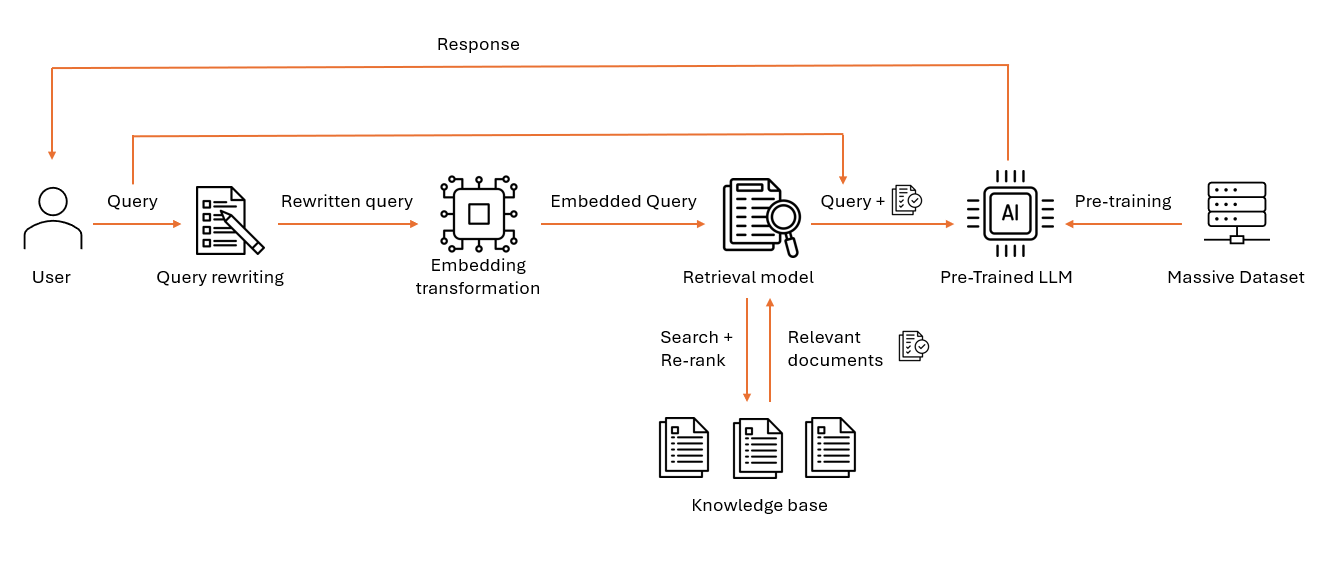
\includegraphics[scale=0.45]{Images/Preliminaries/Retrieval-Augmented Generation Process.png}
\vspace{5mm}
\caption{RAG Process}
\end{figure}

The RAG process is composed of two main components: the retriever and the generator. The retriever is responsible for locating and extracting relevant information from an external knowledge source, employing techniques such as keyword-based search, semantic similarity search, or neural network-based retrieval to ensure precise results. The generator then utilizes the retrieved context to produce coherent and accurate responses, ensuring the output aligns with the user's query while maintaining relevance and context. Together, these components form a robust framework for leveraging external knowledge in generative tasks.
% The retriever focuses on identifying and gathering relevant information from an external knowledge source using methods like keyword search, semantic similarity search, or neural network-based retrieval. The generator focuses on creating accurate responses based on the context retrieved from the retriever. 

% By leveraging embedding models, which convert text into high-dimensional vectors representing semantic meaning, the retriever compares the query against stored embeddings to locate the most relevant data. This ensures that the information retrieved is both contextually appropriate and content-rich, forming a solid foundation for the next phase of the process.

\section{Retriever}

The retriever stage involves finding and gathering relevant text passages from an external knowledge source. This can be done through various methods such as keyword-based search, semantic similarity search, or neural network-based retrieval techniques.
One major application of embedding models is neural retrieval. By measuring the semantic relationship with the text embeddings, allowing for the comparison of text based on content rather than just keyword matching, then the relevant answers to the input query can be retrieved based on the embedding similarity.

\subsection{Preprocessing}
Preprocessing starts with the cleaning and extraction of raw data in diverse formats like PDF, HTML, Word, and Markdown, which is then converted into a uniform plain text format. To accommodate the context limitations of language models, text is segmented into smaller, digestible chunks. Chunks are then encoded into vector representations using an embedding model and stored in a vector database. This step is crucial for enabling efficient similarity searches in the subsequent retrieval phase \cite{gao2023ragllmsurvey}.

There are ways to optimize the indexing process to enhance the performance of the upcoming retrieval steps:
\begin{enumerate}
    \item Chunking strategy: Documents can be splitted into chunks using various methods like fixed-size chunking (for structured documents and surveys), recursive chunking (for documents with large amounts of data), sentence-aware chunking (for analysis of textbooks) and sematic chunking (for information retrieval systems and legal document analysis) \cite{kshirsagar2024chunking}.
    \item Metadata attachments: Each chunk can include extra information (page number, file name, author, category, or timestamp) as metadata. Afterward, the retrieval process can be refined by filtering results based on metadata, which helps narrow down the search. Assigning different weights to document timestamps during retrieval can achieve time-aware RAG, ensuring the freshness of knowledge and avoiding outdated information \cite{gao2023ragllmsurvey}.
\end{enumerate}

\begin{figure}[H]
\centering
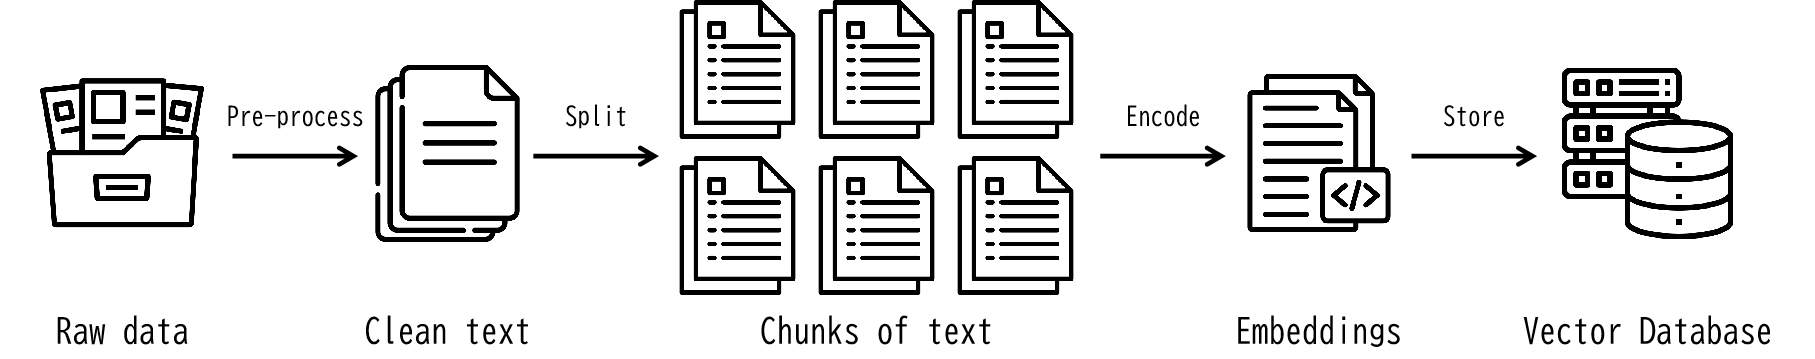
\includegraphics[scale=0.45]{Images/knowledge/indexing.png}
\vspace{5mm}
\caption{Preprocessing process for retriever}
\end{figure}

\subsection{Embedding}
Embeddings are a key component of 
% Retrieval-Augmented Generation (RAG)
RAG systems, which are used to effectively retrieve pertinent information from big datasets. By converting textual data into numerical representations, these embeddings are vector-based representations, typically generated by neural networks, that transform input text into a structured vector space. In this space, proximity reflects the semantic relationships of the input.

In essence, an embedding is a vector, a high-dimensional representation of a text in which every dimension represents a distinct facet of meaning. Consider a two-dimensional Cartesian coordinate system from the algebra class, but with a lot more dimensions (usually 768, 1024, or 1536) to better visualize this. Models such as BERT \cite{devlin2019bert} and Sentence-BERT \cite{reimers-2019-sentence-bert} employ this high-dimensional vector space to represent the semantic features of text. By calculating the distance between these vectors, embeddings enable the system to extract pertinent information from large datasets and choose the most contextually relevant text passages for response generation. This feature is essential for enhancing large language models' (LLMs') outputs' contextual relevance and accuracy.

Many embedding techniques have been used over the years:
\begin{enumerate}
    \item \textbf{Word2Vec} \cite{mikolov2013efficient}: A well-liked technique that uses the Continuous Bag of Words (CBOW) or Skip-gram models to learn word embeddings depending on local context. Word2Vec is effective at many jobs, but it has a major drawback: it has trouble handling polysemy, which is the situation where words have several meanings depending on the context. This is because Word2Vec creates a single representation for every word, independent of how it is used.

    \item \textbf{BERT} \cite{devlin2019bert}: A transformer-based model that generates contextual embeddings, considering both the preceding and following words in a sentence. This allows BERT to produce more accurate representations of words based on their surrounding context. It has been widely adopted for many NLP tasks such as question answering, sentiment analysis, and named entity recognition.

    \item \textbf{Sentence-BERT} (SBERT) \cite{reimers-2019-sentence-bert}: An extension of BERT, fine-tuned specifically for generating sentence embeddings. Unlike traditional BERT, which produces word-level embeddings, SBERT produces fixed-size embeddings for entire sentences. This allows for efficient comparison of sentence pairs, making SBERT highly effective for tasks like semantic textual similarity, paraphrase identification, and information retrieval.

    \item \textbf{FAISS} \cite{douze2024faiss} and \textbf{dense retrieval techniques}: In RAG systems, embeddings are often used with specialized retrieval tools like Facebook AI Similarity Search (FAISS) to perform fast, approximate nearest neighbor search. This helps locate the most relevant pieces of information from a large corpus, making the retrieval process both scalable and efficient.
\end{enumerate}


Moreover, our embedding can be trained in different ways: 
\begin{enumerate}
    \item \textbf{Supervised learning:} In supervised learning, embeddings are trained with labeled data to predict specific outcomes, such as class labels or relationships. Examples include training embeddings for tasks like sentiment analysis or named entity recognition (NER).
    \item \textbf{Unsupervised learning:} Unsupervised learning allows embeddings to be trained without labels, often by predicting words or context from surrounding text. Models like Word2Vec and global vectors for word representation (GloVe) \cite{Pennington2014GloVeGV} use this method to learn semantic relationships between words from large corpora.
   
\end{enumerate}

\textbf{Fine-tune embedding models}: Reinforcement learning \cite{kulkarni2024rag}: In reinforcement learning, embeddings are dynamically adjusted based on feedback from the environment to improve the system's performance over time. For instance, in a RAG system designed for domain-specific chatbots, reinforcement learning is employed to optimize the retrieval of relevant context. Using reinforcement learning with human feedback (RLHF) \cite{kulkarni2024rag}, models like GPT-4 are fine-tuned to respond accurately to domain-specific queries. A key example is optimizing FAQ retrieval for customer service chatbots. In such systems, reinforcement learning is used to decide whether to fetch additional context for each user query or rely on previously retrieved information. The system evaluates the quality of the generated responses (e.g., by GPT-4) and uses this evaluation as a reward signal. For example, if the system correctly answers a follow-up query without fetching redundant FAQ context, it receives a positive reward, thereby learning to minimize unnecessary retrievals. This approach not only improves efficiency by saving computational resources (such as API token usage) but also enhances accuracy by reducing noise in the generated outputs.
% \end{itemize}

\subsection{Hierarchical navigable small world (HNSW) indexing}
\begin{enumerate}
    \item \textbf{Vector database and HNSW:}
\end{enumerate}

In RAG systems, vector database plays a pivotal role in efficiently retrieving relevant information to augment the capabilities of generative language models. These databases are designed to store and query high-dimensional embeddings, which are numerical representations of text, code, images, or other data. Embeddings capture semantic relationships between data points, enabling similarity searches based on meaning rather than exact matches. This makes vector databases a cornerstone of modern RAG pipelines, ensuring that retrieved context aligns with the query’s intent. To achieve efficient and scalable retrieval from large embedding datasets, RAG systems often employ approximate nearest neighbor (ANN) algorithms, with HNSW graphs \cite{malkov2018hnsw} being one of the most widely used techniques.

\begin{enumerate}
    \setcounter{enumi}{1}
    \item \textbf{HNSW algorithm:}
\end{enumerate}
    
The HNSW algorithm is built on the concept of organizing links based on their length scales across multiple layers, enabling efficient search within a hierarchical, multilayer graph structure.

\begin{figure}[H]
    \centering
    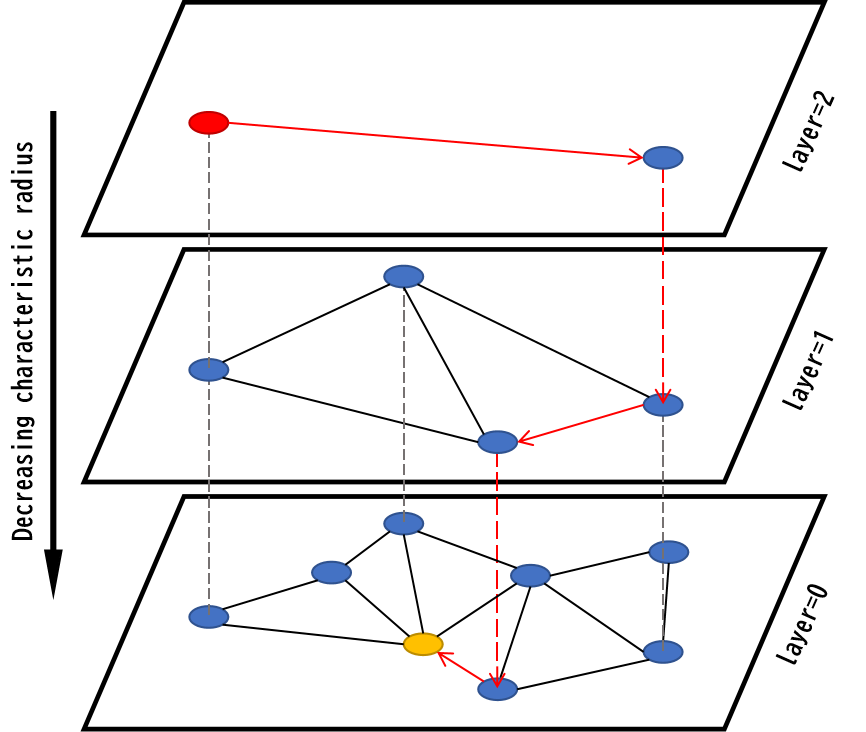
\includegraphics[width=0.4\textwidth]{Images/Preliminaries/hnsw.png}
    \vspace{5mm}
    \caption{HNSW search algorithm visualization. The search starts from entry point from top layer (shown red), red arrows show direction of greedy algorithm to query point (shown yellow) \cite{malkov2018hnsw}.}
    \end{figure}

The HNSW algorithm begins with a network construction phase (Algorithm 1), where the graph structure is incrementally built through the consecutive insertion of stored elements. For each new element, a maximum layer $l$ is randomly determined using an exponentially decaying probability distribution. This hierarchical organization ensures that higher layers contain progressively fewer nodes, optimizing the search process by focusing on coarse-to-fine navigation.

The insertion process begins at the top layer of the hierarchical graph, where the algorithm performs a greedy traversal to locate the $ef$ closest neighbors to the newly inserted element $q$ within that layer. Once these nearest neighbors are identified, they serve as entry points for the next layer. This process is repeated layer by layer, moving downward through the graph, ensuring that the inserted element is effectively connected to its most relevant neighbors at each level.

\begin{algorithm}[H]
\caption{INSERT(\texttt{hsnw}, $q$, $M$, $M_{\text{max}}$, ${efConstruction}$, $mL$)}\label{alg:insert}
\begin{algorithmic}[1]
\Require multilayer graph \texttt{hsnw}, new element $q$, number of established connections $M$, maximum number of connections per element per layer $M_{\text{max}}$, size of the dynamic candidate list ${efConstruction}$, normalization factor for level generation $mL$
\Ensure update \texttt{hsnw} inserting element $q$
\State $W \gets \emptyset$ \Comment{list for the currently found nearest elements}
\State $ep \gets$ get enter point for \texttt{hsnw}
\State $L \gets$ level of $ep$ \Comment{top layer for \texttt{hsnw}}
\State $\ell \gets -\lfloor \ln(\text{unif}(0,1)) \cdot mL \rfloor$ \Comment{new element's level}
\State $\ell \gets \min(\ell, L + 1)$
\For{$\ell{c} \gets L$ \textbf{to} $\ell+1$}
    \State $W \gets$ \texttt{SEARCH-LAYER}$(q, ep, {ef}=1, \ell{c})$
    \State $ep \gets$ get the nearest element from $W$ to $q$
\EndFor
\For{$\ell{c} \gets \min(L, \ell)$ \textbf{to} $0$}
    \State $W \gets$ \texttt{SEARCH-LAYER}$(q, ep, {efConstruction}, \ell{c})$
    \State $\texttt{neighbors} \gets$ \texttt{SELECT-NEIGHBORS}$(q, W, M, \ell{c})$ \Comment{Algorithm 3 or 4}
    \State add bidirectional connections from \texttt{neighbors} to $q$ at layer $\ell{c}$
    \For{each $e \in \texttt{neighbors}$}
        \State $eComm \gets \texttt{neighborhood}(e)$ at layer $\ell{c}$
        \If{$|eComm| > M_{\text{max}}$} \Comment{shrink connections if needed}
            \If{$\ell{c} = 0$} \Comment{if $\ell{c}=0$ then $M_{\text{max}} = M_{\text{max}0}$}
                \State $M_{\text{max}} \gets M_{\text{max}0}$
            \EndIf
            \State $eComm \gets$ \texttt{SELECT-NEIGHBORS}$(e, eComm, M_{\text{max}}, \ell{c})$ \Comment{Algorithm 3 or 4}
        \EndIf
        \State set \texttt{neighborhood}$(e)$ at layer $\ell{c}$ to $eComm$
    \EndFor
\EndFor
\State $ep \gets W$
\State set enter point for \texttt{hsnw} to $q$
\end{algorithmic}
\end{algorithm}

Closest neighbors at each layer are identified using a variant of the greedy search algorithm (as outlined in Algorithm 2). To approximate the $ef$ nearest neighbors at a given layer $l_c$, the algorithm maintains a dynamic list $W$, which stores the $ef$ closest found elements. This list is initially populated with the entry points and is iteratively updated during the search process.

\input{components/contents/hnsw_algo/search_layer}

At each step, the algorithm evaluates the neighborhood of the closest, yet-to-be-evaluated element in $W$. The search continues until the neighborhoods of all elements in $W$ have been evaluated. Unlike traditional approaches that limit the number of distance calculations, the HNSW stop condition offers a key advantage: it discards candidates for evaluation that are farther from the query than the furthest element already in $W$. This approach prevents unnecessary evaluations and avoids bloating the search structures, ensuring a more efficient and streamlined search process.

In the HNSW algorithm, two methods are employed to select M neighbors from a pool of candidates during the graph construction phase: Simple (Algorithm 3) and Heuristic (Algorithm 4).

\begin{algorithm}[H]
\caption{SELECT-NEIGHBORS-SIMPLE($q$, $C$, $M$)}\label{alg:nei_sim}
\begin{algorithmic}[1]
\Require Base element $q$, candidate elements $C$, number of neighbors to return $M$
\Ensure $M$ nearest elements to $q$
\State \textbf{return} $M$ nearest elements from $C$ to $q$
\end{algorithmic}
\end{algorithm}
\begin{algorithm}[H]
\caption{SELECT-NEIGHBORS-HEURISTIC($q$, $C$, $M$, $\ell{c}$, ${extendCandidates}$, ${keepPrunedConnections}$)}\label{alg:nei_heu}
\begin{algorithmic}[1]
\Require Base element $q$, candidate elements $C$, number of neighbors to return $M$, layer number $\ell{c}$, flag indicating whether or not to extend candidate list ${extendCandidates}$, flag indicating whether or not to add discarded elements ${keepPrunedConnections}$
\Ensure $M$ elements selected by the heuristic
\State $R \gets \emptyset$
\State $W \gets C$ \Comment{Working queue for the candidates}
\If{${extendCandidates}$} \Comment{Extend candidates by their neighbors}
    \For{each $e \in C$}
        \For{each $e_{\text{adj}} \in \texttt{neighbourhood}(e)$ at layer $\ell{c}$}
            \If{$e_{\text{adj}} \notin W$}
                \State $W \gets W \cup e_{\text{adj}}$
            \EndIf
        \EndFor
    \EndFor
\EndIf
\State $W_d \gets \emptyset$ \Comment{Queue for the discarded candidates}
\While{$|W| > 0$ \textbf{and} $|R| < M$}
    \State $e \gets$ Extract nearest element from $W$ to $q$
    \If{$e$ is closer to $q$ compared to any element from $R$}
        \State $R \gets R \cup e$
    \Else
        \State $W_d \gets W_d \cup e$
    \EndIf
\EndWhile
\If{${keepPrunedConnections}$} \Comment{Add some of the discarded connections from $W_d$}
    \While{$|W_d| > 0$ \textbf{and} $|R| < M$}
        \State $R \gets R$ $ \cup$ Extract nearest element from $W_d$ to $q$
    \EndWhile
\EndIf
\State \textbf{return} $R$
\end{algorithmic}
\end{algorithm}

The K-approximate nearest neighbor search (K-ANNS) algorithm, as implemented in the HNSW framework, is detailed in Algorithm 5. It is conceptually similar to the insertion process of an item with a designated top layer $l=0$. However, instead of establishing new connections, the goal of the K-ANNS algorithm is to identify and return the closest neighbors in the graph's ground layer as the final search results.

\input{components/contents/hnsw_algo/knn}

\subsection{Pre-retrieval}

\textbf{Query expansion}: In the context of RAG, a single query can be transformed and expanded into multiple variations that are semantically enriched, capturing different nuances and interpretations of the original input. By diversifying the queries, the system increases the likelihood of retrieving contextually specific and relevant information from the knowledge base. This enriched retrieval process ensures that the generated responses are not only more precise but also better aligned with the user's intent, ultimately enhancing the quality and relevance of the output provided by the model \cite{gao2023ragllmsurvey}.

\textbf{Query rewriting}: The original queries are not always optimal for LLM retrieval, especially in real-world scenarios. Therefore, we can prompt LLM to rewrite the queries \cite{gao2023ragllmsurvey}. Query rewriting in RAG refers to the process of refining or reformulating user queries to enhance the retrieval module's effectiveness. This step is critical in ensuring that the retriever fetches highly relevant and accurate documents or context from the knowledge base. Effective query rewriting includes disambiguating vague queries, expanding them with synonyms or related terms, correcting errors, and incorporating historical or contextual information. By improving the quality of the input to the retriever, query rewriting significantly boosts the overall performance of the RAG system, leading to more accurate and contextually appropriate outputs from the generation module. A user query can be transformed and decomposed in many ways before being executed as part of a RAG query engine, agent, or any other pipeline.\\\
\begin{figure}[H]
\vspace{2pt}
\centering
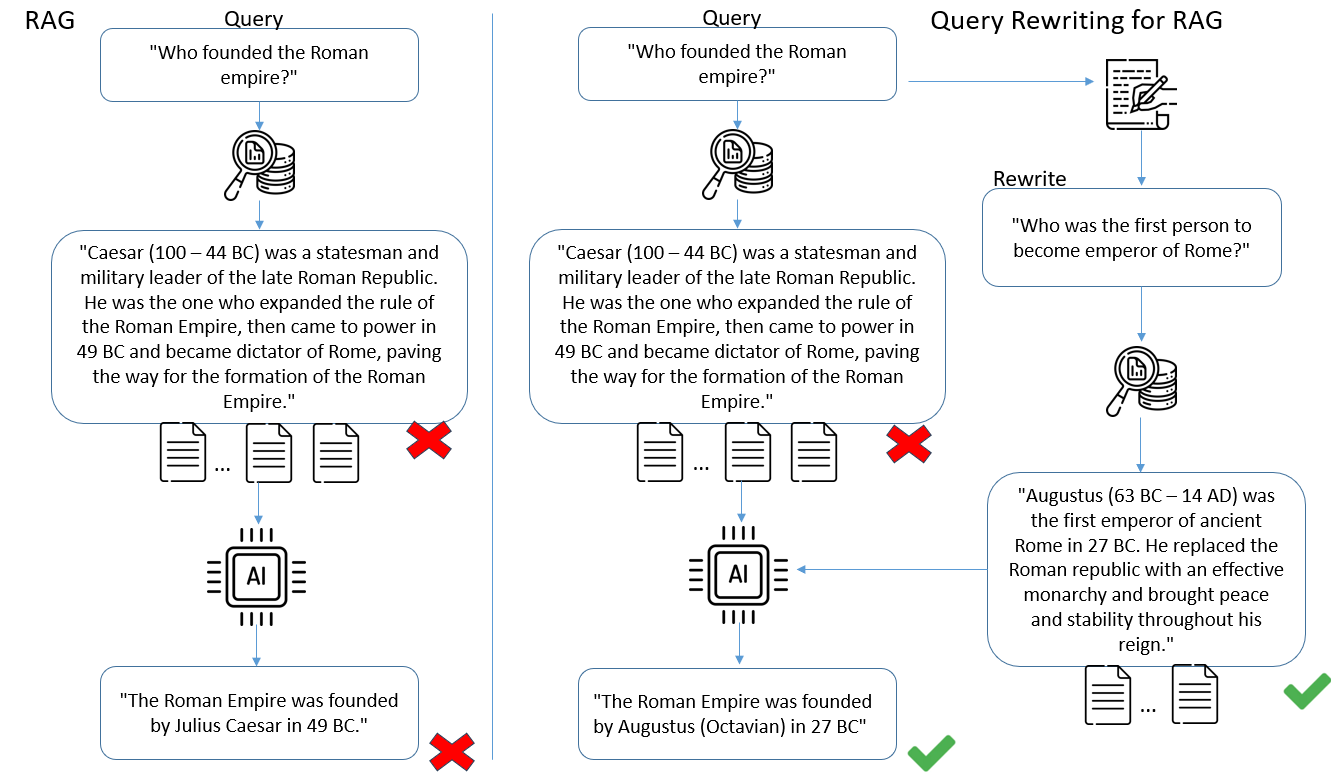
\includegraphics[scale=0.45]{Images/Preliminaries/Query_Rewriting.png}
\vspace{5mm}
\caption{Query rewriting process in RAG}
\end{figure}

\textbf{Embedding transformation}: involves either pretraining language models or leveraging pretrained models to gain a deep understanding of the structural and semantic characteristics of text data. This process enables language models to map both queries and structured texts into one unified embedding space, facilitating efficient and accurate retrieval \cite{li2023santa}. By doing so, the model enables efficient and accurate retrieval by ensuring that semantically related information from different formats is aligned within the same representation space. This unified embedding not only improves retrieval precision but also facilitates the integration of heterogeneous knowledge sources into the retrieval process.


% \begin{itemize}
%     \item A task with retrieval augmentation can be described as follows:\\
% Given a dataset for a knowledge-intensive task (e.g., open-domain QA), 
% \[ D = \{(x, y)_i\}, \, i = 0, 1, 2, \dots, N \]
% where \( x \) (e.g., a question) is the input to the pipeline, and \( y \) is the expected output (e.g., the correct answer), the pipeline operates in three main steps:

% \begin{enumerate}
%     \item \textbf{Query Rewrite:} Reformulate the original query \( x \) into another form to better retrieve relevant passages \( \tilde{x} \). We strive to develop an improved rewrite model, $M_\theta$, capable of transforming the original query $x$ into a rewritten form, expressed as:
%     \[
%     \tilde{x} = M_\theta(x),
%     \]
%     \item \textbf{Retrieve:} where \( \tilde{x} \) represents the reformulated query, which serves as the basis for retrieving a refined set of documents $D'$, essential for completing the downstream task. 
%     \item \textbf{Read:} Comprehend the input along with the retrieved contexts \([D', x]\) and predict the output \( \hat{y} \).
% \end{enumerate}

% A straightforward but effective approach involves using a large language model (LLM) to rewrite queries to retrieve potentially relevant information. A few-shot prompt is employed to encourage the LLM to "think" about the task. The output can be none, one, or multiple queries, which are then used to perform the search.
% \item Techniques for Query Rewriting:
% \begin{enumerate}
%     \item Query rewriting: Make queries more specific and detailed, improving the probability of retrieving the most relevant information
%     \item Step-back prompting: Generate broader and more general queries that can help retrieve relevant background information
%     \item Sub-query decomposition: Break down complex queries into simpler sub-queries for more comprehensive information retrieval.
% \end{enumerate}

% Few-Shot Prompting:

% Use LLMs with few-shot prompts to generate high-quality rewritten queries without extensive training.
%     \item Query Rewriting using QueryTransform code example:
% \begin{lstlisting}
% from llama_index.core.indices.query.query_transform import HyDEQueryTransform
% from llama_index.llms.openai import OpenAI

% hyde = HyDEQueryTransform(include_original=True)
% llm = OpenAI(model="gpt-3.5-turbo")

% query_bundle = hyde.run("What is Bel?")
% \end{lstlisting}
% This generates a query bundle that contains the original query, but also $custom_embedding_strs$ representing the queries that should be embedded.
% \end{itemize}

\subsection{Retrieval}

Once the embedding process is complete, a document retrieval system identifies and returns the most relevant documents based on the query. In a RAG pipeline, this document retrieval step plays a crucial role, supplying the LLM with the appropriate documents for generating contextually accurate responses. Formally, given a query $q$ in an arbitrary language $x$, it can retrieve document $d$ in language $y$ (which can be another language or the same language as $x$) from the corpus $D^y$. Moreover, the retrieval function $fn^*()$ belongs to any of the functions: dense, lexical, or multi-vector retrieval \cite{chen2024bge}.
\begin{center}
    $d^y \leftarrow {\rm{fn}}^*(q^x, D^y)$
\end{center}
\begin{itemize}
    \item \textbf{Dense retrieval} \\\\
Query $q$ is transformed into the hidden states $H_q$ based on a text encoder.

The normalized hidden state of the special token "[CLS]" is used for the representation of the query:
$$ e_q = \text{norm}(H_q[0]) $$

Similarly, the embedding of passage $p$ is:
$$ e_p = \text{norm}(H_p[0]) $$

The relevance score between query and passage is measured by the inner product between the two embeddings $e_q$ and $e_p$
$$ s_{dense} \leftarrow \langle e_p, e_q \rangle $$
    \item \textbf{Lexical retrieval}\\\\
For each term \textbf{t} in the query:

$$ w_{q_t} \leftarrow \text{ReLU}(W^T_{lex} H_q[i]) $$

Similarly, for the passage:

$$ w_{p_t} \leftarrow \text{ReLU}(W^T_{lex} H_p[i]) $$

Where:

- $W_{lex} \in R^{d \times 1}$: A weight matrix mapping the hidden state to a scalar.

- $H_q[i]$, $H_p[i]$: Hidden states (embedding vectors) for the $i$-th token in the query and passage.

- ReLU: Rectified Linear Unit activation function, defined as $\text{ReLU}(x) = \max(0, x)$.
    \item \textbf{Multi-vector retrieval}\\\\
Representing query and passage with multiple vectors

Formulas:

- Query representation:  
  $$ E_q = \text{norm}(W_{mul}^\top H_q) $$

- Passage representation:  
  $$ E_p = \text{norm}(W_{mul}^\top H_p) $$

- $W_{mul} \in \mathbb{R}^{d \times d}$: A learnable projection matrix.

- $H_q$ and $H_p$: Hidden states (embeddings) for the query and passage, respectively.

- norm: Column-wise normalization function applied to each vector in the matrices.
\end{itemize}

\subsection{Post-retrieval}

\textbf{Reranking}: The initial retrieval stage often relies on methods like dense or lexical retrieval, which are efficient but may not consistently yield highly relevant documents. To address this, reranking plays a crucial role by reorganizing the retrieved documents to better align with the given query, thereby improving their relevance.\\

\textbf{Contextual compression}: Contextual compression addresses the challenge of retrieving relevant information from large documents by compressing and filtering content based on the query. Instead of passing entire documents, which can lead to expensive and less effective responses, this approach refines the retrieved results. Using a base retriever and a document compressor tools like Compact \cite{yoon2024compact}, it will shortens documents by extracting only the relevant content or removing irrelevant ones entirely, ensuring more efficient and focused query responses.

\section{Generator}
% RNN \cite{rumelhart1988rnn}
% LSTM \cite{lstm}

The posed query and selected documents are synthesized into a coherent prompt to which a large language model is tasked with formulating a response. The model’s approach to answering may vary depending on task-specific criteria, allowing it to either draw upon its inherent parametric knowledge or restrict its responses to the information contained within the provided documents. In cases of ongoing dialogues, any existing conversational history can be integrated into the prompt, enabling the model to engage in multi-turn dialogue interactions effectively  \cite{gao2023ragllmsurvey}.

% Several foundational architectures can be used for RAG's generator like RNN \cite{rumelhart1988rnn}, LSTM Network \cite{lstm} and Transformer \cite{vaswani2017}. In this section, we will introduce RNN, LSTM and Sequence-to-Sequence Architecture \cite{seq2seq}, then we introduce Transformer models.

In this section, we provide an overview of the architecture of Transformer models \cite{vaswani2017} and delve into their core mechanisms that have revolutionized natural language processing. Following this, we explore various prompt engineering techniques, highlighting their role in optimizing the performance of pre-trained language models across a wide range of tasks, including RAG. These techniques not only improve the model's understanding of task-specific contexts but also enhance its ability to generate accurate and contextually relevant responses.

% \subsection{RNN \& LSTM}

% \subsection{Sequence-to-Sequence}

\subsection{Transformer architecture}

Transformer \cite{vaswani2017}, a model architecture eschewing recurrence and instead relying entirely on an attention mechanism to draw global dependencies between input and output \cite{vaswani2017}. It has revolutionized natural language processing (NLP) by enabling parallel processing of sequences. Unlike recurrent architectures such as RNNs \cite{rumelhart1988rnn} or LSTMs \cite{lstm}, which process inputs sequentially and struggle with long-range dependencies, Transformers use self-attention mechanisms to focus on relevant parts of the input across the entire sequence simultaneously. This approach not only improves the ability to capture intricate relationships within the data but also drastically increases computational efficiency by enabling systems to handle tasks in parallel. The result is a model architecture that excels at tasks requiring a deep understanding of context, from machine translation to text generation, setting the foundation for state-of-the-art language models like GPT \cite{radford2018GPT}, BERT \cite{devlin2019bert}, and T5 \cite{raffel2023t5}.

\textbf{Encoder and decoder stacks}: A transformer consists of two components: encoder and decoder. Each of them is a stack of N identical layers (N=6 in the original transformer model).
\begin{itemize}
    \item \textbf{Encoder}: The encoder is composed of a stack of N identical layers. Each layer has two sub-layers. The first is a multi-head self-attention mechanism, and the second is a simple, position-wise fully connected feed-forward network. Around each of the two sub-layers, there is a residual connection \cite{he2016residualcon} followed by layer normalization \cite{ba2016layernorm}. That is, the output of each sub-layer is $\text{LayerNorm}(x + \text{Sublayer}(x))$, where $\text{Sublayer}(x)$ is the function implemented by the sub-layer itself \cite{vaswani2017}.
    \item \textbf{Decoder}: The decoder, like the encoder, is also composed of a stack of N identical layers. In addition to the two sub-layers in each encoder layer, the encoder inserts a third sub-layer, which performs multi-head attention over the output of the encoder Stack. The the self-attention sub-layer in the decoder stack is modified to prevent positions from attending to subsequent positions. This masking, combined with fact that the output embeddings are offset by one position, ensures that the predictions for position i can depend only on the known outputs at positions less than i \cite{vaswani2017}.
\end{itemize}

\textbf{Positional encoding}: plays a critical role in capturing the order of sequences, which is essential for preserving the structural integrity of text data. Positional encodings are added to the input embeddings at the initial layers of both the Encoder and Decoder stacks, enabling the model to incorporate sequential information. 

In the original model, sine and cosine functions of different frequencies is used for positional encoding:
    
\begin{equation}\label{Eq:PE_sin}
    \text{PE}(pos,2i)=\sin(pos/{10000^{2i/d_{model}}}) 
\end{equation}
\begin{equation}\label{Eq:PE_cos}
    \text{PE}(pos,2i+1)=\cos(pos/{10000^{2i/d_{model}}})
\end{equation}
where $pos$ is the position and $i$ is the dimension. That is, each dimension of the positional encoding corresponds to a sinusoid \cite{vaswani2017}.

\textbf{Self-attention mechanism:}
\begin{itemize}
    \item \textbf{Queries, keys and values}: In self-attention mechanism, transformer compute output by mapping a query with a set of key-value pairs. The output is computed as a weighted sum of the values, where the weight computed by scaled dot-product of query and keys.
    \item \textbf{Scaled-dot products}: The concept of self-attention lies in computing a weighted sum of values, where the weights represent the similarity between queries and keys. In Transformers, this similarity is determined using a dot product between the query and key vectors, followed by a softmax function. The softmax operation normalizes these weights, ensuring they fall within the range of 0 and 1, thus effectively controlling their influence. 
    \item The vectors for queries, keys, and values are all of size $\color{black}d_K$. When computing the dot product between queries and keys, the resulting values can become disproportionately large, especially as $\color{black}d_K$ increases. Such large values can cause gradients to vanish during backpropagation, hindering the training process. To mitigate this, transformers introduce a scaling factor $\color{black}\sqrt{d_K}$, dividing the dot product by this value. This adjustment helps stabilize the gradients and ensures the training remains efficient and effective, even with large vector dimensions.

\begin{equation}\label{Eq:scale-dot-att}\textcolor{black}
    {\rm{Attention}}(Q,K,V)={\rm{softmax}}(\frac{QK^T}{\sqrt{d_K}}V)
\end{equation}

\begin{figure*}[h!]
    \centering
    % \captionsetup{width=\linewidth}
    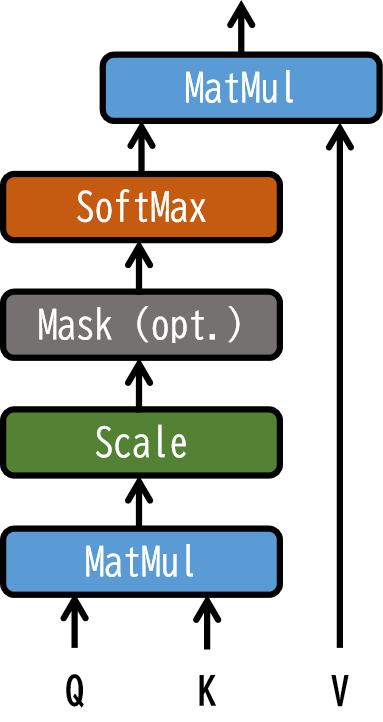
\includegraphics[scale = 0.5]{Images/Preliminaries/transformers/scale-dot-attention.png}
    \vspace{5mm}
    \caption{Scaled dot-product attention \cite{vaswani2017}.}
    \label{fig:scale-dot-attention}
\end{figure*}

    \item \textbf{Multi-head attention}:
    Instead of performing a single attention function with keys, values and queries, it is good to linearly project the queries, keys and values h times with different, learned linear projections to $\color{black}d_k$, $\color{black}d_k$ and $\color{black}d_v$ dimensions, respectively. On each of these projected versions of queries, keys and values we then perform the attention function in parallel. Here, $W^Q_i \,W^K_i\in R^{d_{model}\times d_V},W^Q_i\in R^{d_{model}\times d_V}, W^O \in R^{hd_{v}\times d_{model}}$ and $h$ is the number of attention heads.
\begin{equation}\label{Eq:multi-head-att}
\begin{split}
    \text{MultiHead}(Q,K,V) &= \text{Concat}(head_1, ..., head_h)W^O \\
    & \text{where} \, head_i=\text{Attention}(QW^Q_i,KW^K_i,VW^V_i)\\
\end{split}
\end{equation}

\begin{figure}[h!]
    \centering
    % \captionsetup{width=\linewidth}
    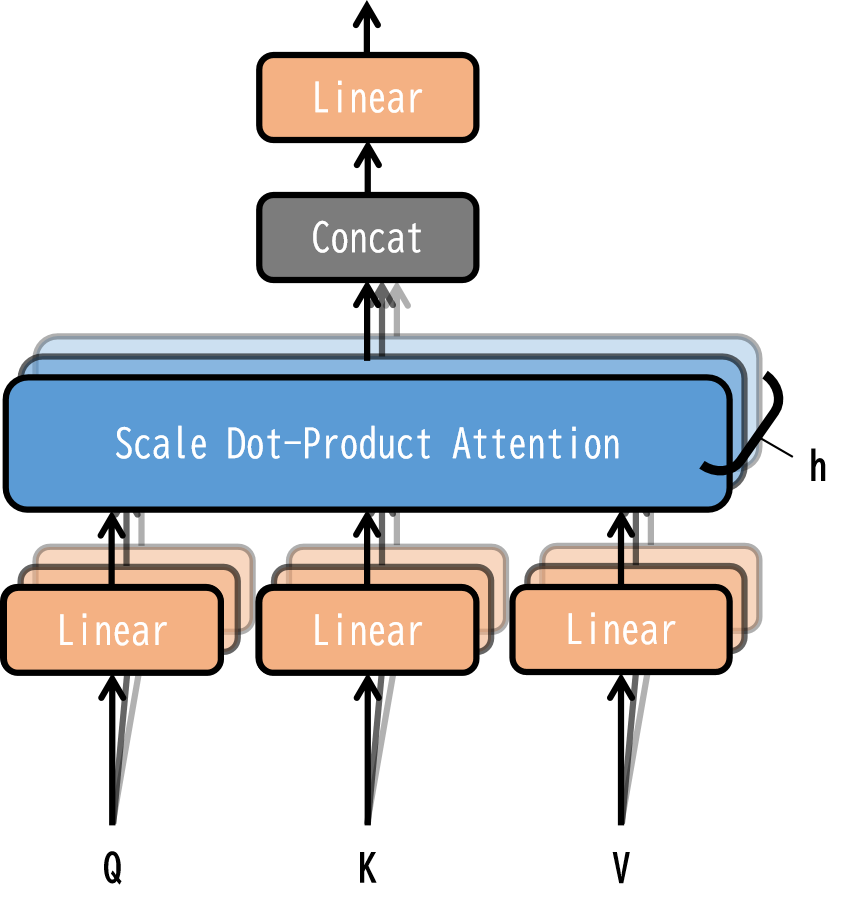
\includegraphics[scale = 0.4]{Images/Preliminaries/transformers/multi-head-attention.png}
    \vspace{5mm}
    \caption{Multi-Head Attention (consists of several attention layers running in parallel) \cite{vaswani2017}.}
    \label{fig:multi-head-attention}
\end{figure}
\end{itemize}

\subsection{Prompt engineering}

Prompt engineering is an essential methodology for maximizing the potential of pre-trained language models. It focuses on carefully crafting task-specific instructions, known as prompts, to direct the model's output effectively without requiring any modifications to its underlying parameters \cite{surveypromptengineering}. Various techniques have been developed to refine the practice of prompt engineering, each aimed at leveraging the full potential of pre-trained language models for diverse and complex applications. Among the most prominent methods are:
\begin{itemize}
    \item \textbf{Zero-Shot (0S) prompting}: This technique involves providing the model with a clear and specific instruction for a task without any prior examples. This method provides maximum convenience, potential for robustness, and avoidance of spurious correlations \cite{fewshot}. Zero-shot prompting relies entirely on the model's pre-trained knowledge and ability to generalize across contexts, making it effective for a wide range of tasks without additional data.
    \item \textbf{Few-Shot (FS) prompting}: This method works by giving K examples (with K often ranging from 10 to 100) of context and completion, and then one final example of context, then the model is expected to provide the final completion \cite{fewshot}. These K examples act as a guide for the model, helping it understand the structure, context, or desired behavior for the task.
    \item \textbf{One-Shot (1S) prompting}: This approach is the same as FS prompting but only one example is used for the prompt. This way of prompting closely matches the way in which some tasks are communicated to humans \cite{fewshot}, normally we are given one single example or demonstration of the task then we are asked to complete other similar tasks.
    \item \textbf{Chain-of-Thought (CoT) prompting}: This technique involves prompting a coherent series of intermediate reasoning steps that lead to the final answer for a problem rather than providing a direct answer \cite{chainofthought}. By simulating a logical progression of thought, the model is better equipped to handle complex tasks that require multi-step reasoning, such as mathematical problem-solving or logical deductions. This structured guidance fosters greater accuracy and depth in responses.
    % \item \textbf{Tree-of-Thought (ToT) Prompting}

\end{itemize}


% Choosing a proper prompt has a large effect not only on accuracy but also on which task the model performs in the first place \cite{promptingmethods}.

% \end{itemize}

% \subsubsection{Information Compression}
% \subsubsection{Reranking}

\section{Augmentation methods}

\subsection{Augmentation stage: Inference}

At the inference stage, augmentation involves retrieving and integrating external knowledge dynamically during the generation process. Recent work, such as in-context RALM \cite{ram2023incontext}, demonstrates the efficacy of prepending retrieved documents to the input text without modifying the language model (LM) architecture. This approach leverages off-the-shelf retrievers for document selection, providing significant performance gains while maintaining simplicity.

Language models define probability distributions over sequences of tokens. Given such a sequence \(x_1, ..., x_n\), the standard way to model its probability is via next-token prediction:

\[
{\rm{p}}(x_1, ..., x_n) = \prod_{i=1}^{n} {\rm{p}}(x_i | x_{<i}),
\]

where \(x_{<i} := x_1, ..., x_{i-1}\) is the sequence of tokens preceding \(x_i\), also referred to as its prefix. This autoregressive model is usually implemented via a learned transformer network \cite{vaswani2017} parameterized by the set of parameters \(\theta\):

\[
{\rm{p}}(x_1, ..., x_n) = \prod_{i=1}^{n} {\rm{p}}_{\theta}(x_i | x_{<i}).
\]

Retrieval-augmented language models (RALMs) add an operation that retrieves one or more documents from an external corpus \(C\), and conditions the above LM predictions on these documents. Specifically, for predicting \(x_i\), the retrieval operation from \(C\) depends on its prefix \({RC(x_{<i})}\), giving rise to the general RALM decomposition:

\[
{\rm{p}}(x_1, ..., x_n) = \prod_{i=1}^{n} {\rm{p}}(x_i | x_{<i}, RC(x_{<i})).
\]

In-context RALM refers to a simple method of concatenating the retrieved documents within the transformer's input before the prefix, without altering the LM weights \(\theta\):

\[
{\rm{p}}(x_1, ..., x_n) = \prod_{i=1}^{n} {\rm{p}}_{\theta}(x_i | [RC(x_{<i}); x_{<i}]),
\]

where \([a; b]\) denotes the concatenation of strings \(a\) and \(b\). This approach allows the model to incorporate external knowledge efficiently.

Two practical design choices in RALM systems significantly impact performance:

\begin{enumerate}
    \item \textbf{Retrieval stride: } 
       Retrieval operations can be performed once every \(s > 1\) tokens to reduce computation costs. The retrieval stride \(s\) determines how often new documents are fetched, trading runtime for performance. The formulation becomes:
   \[
   {\rm{p}}(x_1, ..., x_n) = \prod_{j=0}^{\lfloor n/s \rfloor - 1} \prod_{i=1}^{s} {\rm{p}}_{\theta}(x_{s \cdot j + i} | RC(x_{\leq s \cdot j}); x_{<(s \cdot j + i)}).
   \]
   \item \textbf{Retrieval query length: }
      The retrieval query at stride \(j\) is typically restricted to the last \(\ell\) tokens of the prefix (\({\rm{p}}_j^{s,\ell} := x_{s \cdot j - \ell + 1}, ..., x_{s \cdot j}\)) to avoid diluting the relevance of the information. The resulting formulation is:

   \[
   {\rm{p}}(x_1, ..., x_n) = \prod_{j=0}^{\lfloor n/s \rfloor - 1} \prod_{i=1}^{s} {\rm{p}}_{\theta}(x_{s \cdot j + i} | [RC(q_j^{s,\ell}); x_{<(s \cdot j + i)}]).
   \]
\end{enumerate}

\begin{figure}[H]
    \centering
    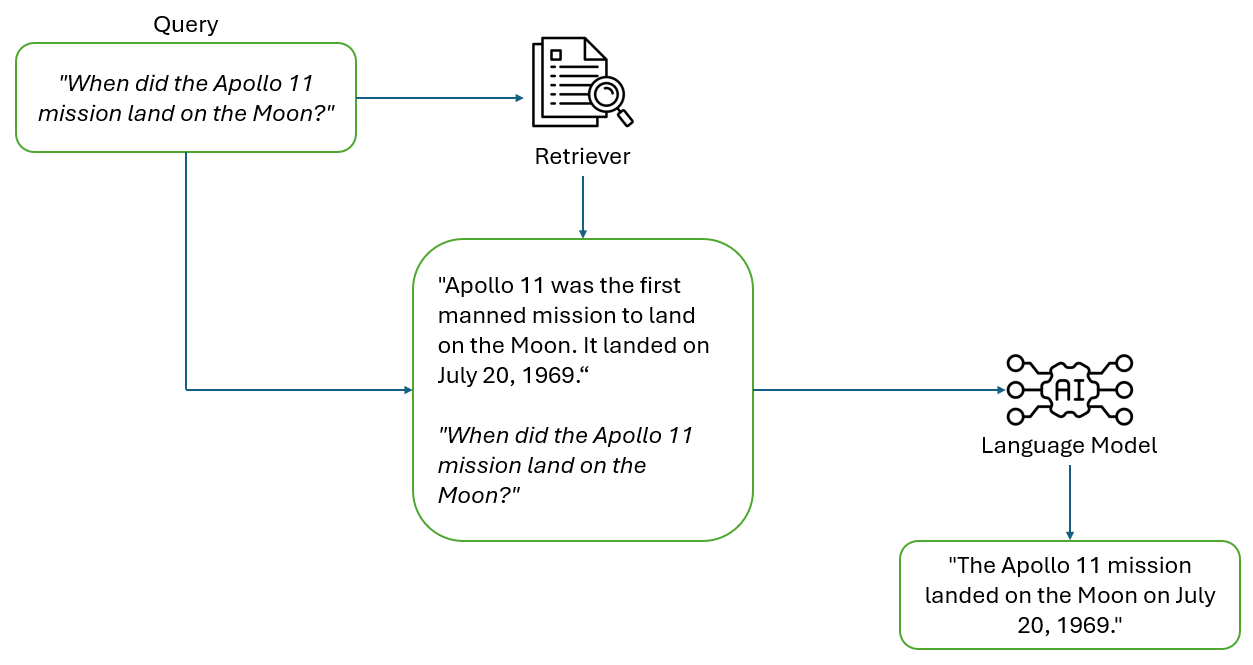
\includegraphics[width=0.8\textwidth]{Images/Preliminaries/Inference stage.png}
    \vspace{5mm}
    \caption{Augmentation during the inference stage. Relevant documents are retrieved and prepended to the input for improved factual grounding.}
\end{figure}

\subsection{Augmentation source: Structured data}

Structured data, such as knowledge bases (KBs), offers a rich source for augmentation. The KnowledGPT framework \cite{wang2023knowledgpt} demonstrates how LLMs can interact with KBs for both retrieval and storage. By generating programmatic queries, LLMs can navigate multi-hop and entity-specific questions effectively.

\begin{figure}[H]
    \centering
    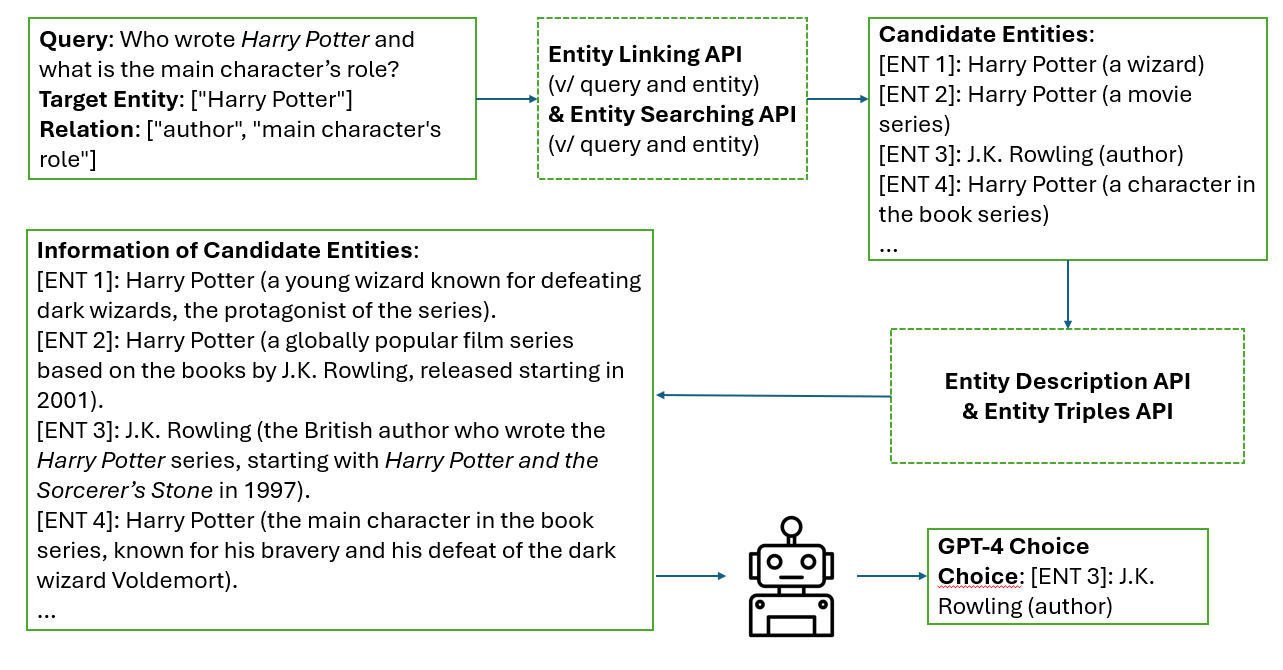
\includegraphics[width=0.8\textwidth]{Images/Preliminaries/Augmentation with structured data.png}
    \vspace{3mm}
    \caption{Workflow of augmentation with structured data sources \cite{wang2023knowledgpt}.} 
\end{figure}

To enable effective interaction with structured data, KnowledGPT employs several key functions:
\begin{itemize}
    \item \textit{get\_entity\_info:} Retrieves encyclopedic descriptions of an entity from the KB.
    \item \textit{find\_entity\_or\_value:} Extracts entities or attribute values related to a query by identifying the most relevant relation.
    \item \textit{find\_relationship:} Identifies relationships between two entities within the KB.
\end{itemize}

These functions allow KnowledGPT to leverage the structured nature of KBs to extract precise and relevant knowledge.

The \textit{find\_entity\_or\_value} function is central to querying entities and attribute values. It matches the query's relation to KB triples using embedding-based similarity and retrieves the corresponding entities or values. The algorithm is detailed below.

\begin{algorithm}
\caption{\text{find\_entity\_or\_value}} \label{alg:cap}
\textbf{Input:} query $q$, alias list of entity $\mathcal{E}$, alias list of relation $\mathcal{R}$. \\
\textbf{Output:} a list of target entities or attribute values $\mathcal{T}$.
\begin{algorithmic}[1]
\Function{\texttt{EMBSIM}}{\textit{str} $r$, \textit{list[str]} $ \mathcal{R}$}
    \State $s = -1$
    \State $r =$ \texttt{embedding}($r$)
    \For{$r_i \in \mathcal{R}$}
        \State $r_i =$ \texttt{embedding}($r_i$)
        \If{$\cos(r, r_i) > s$}
            \State $s = \cos(r, r_i)$
        \EndIf
    \EndFor
    \State \Return $s$
\EndFunction
\State $e =$ \texttt{entity\_linking}($\mathcal{E}$)
\If{$e == NULL$}
    \State \Return $NULL$
\EndIf
\State $r = NULL$
\State $s_r = -1$
\For{$triple$ $\in$ $triples$}
    \State $r_i = $  $triple.rel$
    \State $s_i =$ \Call{\texttt{EMBSIM}}{$r_i, \mathcal{R}$}
    \If{$s_i > s_r$}
        \State $s_r = s_i$
        \State $r = r_i$
    \EndIf
\EndFor
\If{$r == NULL$}
    \State \Return $NULL$
\EndIf
\State $triples_r$ = $triples$ with relation $r$
\State $\mathcal{R}$ = target entities or attribute values in $triples_r$
% \State \textbf{Filter:} Remove any $0$ from $\mathcal{R}$
\State \Return $\mathcal{R}$ % (filtered)
\end{algorithmic}
\end{algorithm}

\subsection{Augmentation process}

The augmentation process in RAG frameworks can be categorized into various types, such as once, iterative, recursive, and adaptive. Among these, the Self-reflective retrieval-augmented generation (SELF-RAG) \cite{asai2023selfrag} approach employs an adaptive process where the model dynamically determines the necessity of retrieval, evaluates the relevance and support of retrieved passages, and critiques its own output for factuality and quality. 

Reflection tokens are special tokens used by SELF-RAG to evaluate and guide the retrieval and generation process.

\begin{table}[H]
\begin{tabular}{c c m {5cm} m {7cm}} 
 \hline
 Type & Input & Output & Definitions \\ [0.5ex] 
 \hline
 Retriever & $x / x, y$ & \{yes, no, continue\} & Decide to Retrieve with $\mathcal{R}$ \\ 
 IsREL & $x, d$ & \{\textbf{relevant}, irrelevant \} & $d$ provide useful information to solve $x$\\
 IsSUP & $x, d, y$ & \{\textbf{fully supported}, partially supported, no support\} & All of the verification-worthy statement in $y$ is supported by d \\
 IsUSE & $x, y$ & \{5, 4, 3, 2, 1\} & $y$ is useful response to $x$ \\ [1ex] 
 \hline
\end{tabular}
\caption{Reflection tokens \cite{asai2023selfrag}.}
% '''''
\end{table}

The inference process in SELF-RAG leverages reflection tokens to dynamically retrieve relevant passages and critique the model's outputs. The steps are as follows:

\begin{enumerate}
    \item \textbf{Input and prediction:} The model receives the input prompt \(x\) and preceding generation \(y<t\). It predicts whether retrieval is necessary using the retrieve token.
    \item \textbf{Retrieve:} If retrieval is needed (retrieve = yes), the retriever fetches relevant passages \(D\) based on the input and context.
    \item \textbf{Generate and evaluate:} For each retrieved passage \(d \in D\), the model:
    \begin{itemize}
        \item Predicts IsREL to assess relevance.
        \item Generates the next segment \(y_t\).
        \item Predicts IsSUP and IsUSE to evaluate support and utility.
    \end{itemize}
    \item \textbf{Rank and select:} The model ranks all generated segments based on IsREL, IsSUP, and IsUSE, and selects the top-ranked segment.
    \item \textbf{No retrieval case:} If retrieval is not needed (Retrieve = no), the model directly generates the next segment and predicts its utility.
    \item \textbf{Iterative refinement:} The process repeats until the response is complete.
\end{enumerate}

\begin{algorithm}
\renewcommand{\algorithmicrequire}{\textbf{Require}}
\caption{SELF-RAG inference}\label{alg:cap1}
\begin{algorithmic}[1]
\Require Generator LM $\mathcal{M}$, Retriever $\mathcal{R}$, Large-scale passage collections $\{d_1, \ldots, d_N\}$
% \Ensure $y = x^n$
\State \textbf{Input:} input prompt $x$ and preceding generation $y_{<t}$, \textbf{Output:} next output segment $y_t$
\State $\mathcal{M}$ predicts Retriever given $(x, y_{<t})$
\If{Retriever == Yes}
    \State Retrieve relevant text passages $\mathcal{D}$ using $\mathcal{R}$ given $(x, y_{t-1})$  \Comment{Retrieve}
    \State $\mathcal{M}$ predicts IsREL given $x, d$ and $y_{<t}$ for each $d \in \mathcal{D}$ \hfill \Comment{Generate}
    \State $\mathcal{M}$ predicts IsSUP and IsUSE given $x, d$ for each $d \in \mathcal{D}$ \hfill \Comment{Critique}
    \State Rank $y_t$ based on IsREL, IsSUP, IsUSE
\ElsIf{Retriever == No}
    \State $\mathcal{M}_{\text{gen}}$ predicts $y_t$ given $x$ \hfill \Comment{Generate}
    \State $\mathcal{M}_{\text{gen}}$ predicts IsUSE given $x, y_t$ \hfill \Comment{Critique}
\EndIf
\end{algorithmic}
\end{algorithm}

% \begin{algorithm}
% \caption{INSERT(\texttt{hsnw}, $q$, $M$, $M_{\text{max}}$, \texttt{efConstruction}, $mL$)}
% \begin{algorithmic}[1]
% \Require multilayer graph \texttt{hsnw}, new element $q$, number of established connections $M$, maximum number of connections per element per layer $M_{\text{max}}$, size of the dynamic candidate list \texttt{efConstruction}, normalization factor for level generation $mL$
% \Ensure update \texttt{hsnw} inserting element $q$
% \State $W \gets \emptyset$ \Comment{list for the currently found nearest elements}
% \State $ep \gets$ get enter point for \texttt{hsnw}
% \State $L \gets$ level of $ep$ \Comment{top layer for \texttt{hsnw}}
% \State $l \gets -\lfloor \ln(\text{unif}(0,1)) \cdot mL \rfloor$ \Comment{new element's level}
% \State $l \gets \min(l, L + 1)$
% \For{$lc \gets L$ \textbf{to} $l+1$}
%     \State $W \gets$ \texttt{SEARCH-LAYER}$(q, ep, \texttt{ef}=1, lc)$
%     \State $ep \gets$ get the nearest element from $W$ to $q$
% \EndFor
% \For{$lc \gets \min(L, l)$ \textbf{to} $0$}
%     \State $W \gets$ \texttt{SEARCH-LAYER}$(q, ep, \texttt{efConstruction}, lc)$
%     \State $\texttt{neighbors} \gets$ \texttt{SELECT-NEIGHBORS}$(q, W, M, lc)$ \Comment{Algorithm 3 or 4}
%     \State add bidirectional connections from \texttt{neighbors} to $q$ at layer $lc$
%     \For{each $e \in \texttt{neighbors}$}
%         \State $eComm \gets \texttt{neighborhood}(e)$ at layer $lc$
%         \If{$|eComm| > M_{\text{max}}$} \Comment{shrink connections if needed}
%             \If{$lc = 0$} \Comment{if $lc=0$ then $M_{\text{max}} = M_{\text{max}0}$}
%                 \State $M_{\text{max}} \gets M_{\text{max}0}$
%             \EndIf
%             \State $eComm \gets$ \texttt{SELECT-NEIGHBORS}$(e, eComm, M_{\text{max}}, lc)$ \Comment{Algorithm 3 or 4}
%         \EndIf
%         \State set \texttt{neighborhood}$(e)$ at layer $lc$ to $eComm$
%     \EndFor
% \EndFor
% \State $ep \gets W$
% \State set enter point for \texttt{hsnw} to $q$
% \end{algorithmic}
% \end{algorithm}

% \begin{algorithm}
% \caption{SEARCH-LAYER($q$, $ep$, $ef$, $lc$)}
% \begin{algorithmic}[1]
% \Require Query element $q$, enter points $ep$, number of nearest to $q$ elements to return $ef$, layer number $lc$
% \Ensure $ef$ closest neighbors to $q$
% \State $v \gets ep$ \Comment{Set of visited elements}
% \State $C \gets ep$ \Comment{Set of candidates}
% \State $W \gets ep$ \Comment{Dynamic list of found nearest neighbors}
% \While{$|C| > 0$}
%     \State $c \gets$ Extract nearest element from $C$ to $q$
%     \State $f \gets$ Get furthest element from $W$ to $q$
%     \If{\texttt{distance}$(c, q) > \texttt{distance}(f, q)$}
%         \State \textbf{break} \Comment{All elements in $W$ are evaluated}
%     \EndIf
%     \For{each $e \in \texttt{neighbourhood}(c)$ at layer $lc$} \Comment{Update $C$ and $W$}
%         \If{$e \notin v$}
%             \State $v \gets v \cup e$
%             \State $f \gets$ Get furthest element from $W$ to $q$
%             \If{\texttt{distance}$(e, q) < \texttt{distance}(f, q)$ \textbf{or} $|W| < ef$}
%                 \State $C \gets C \cup e$
%                 \State $W \gets W \cup e$
%                 \If{$|W| > ef$}
%                     \State Remove furthest element from $W$ to $q$
%                 \EndIf
%             \EndIf
%         \EndIf
%     \EndFor
% \EndWhile
% \State \textbf{return} $W$
% \end{algorithmic}
% \end{algorithm}

% \begin{algorithm}
% \caption{SELECT-NEIGHBORS-SIMPLE($q$, $C$, $M$)}
% \begin{algorithmic}[1]
% \Require Base element $q$, candidate elements $C$, number of neighbors to return $M$
% \Ensure $M$ nearest elements to $q$
% \State \textbf{return} $M$ nearest elements from $C$ to $q$
% \end{algorithmic}
% \end{algorithm}

% \begin{algorithm}
% \caption{SELECT-NEIGHBORS-HEURISTIC($q$,$C$,$M$,$lc$,\texttt{extendCandidates},\texttt{keepPrunedConnections})}
% \begin{algorithmic}[1]
% \Require Base element $q$, candidate elements $C$, number of neighbors to return $M$, layer number $lc$, flag indicating whether or not to extend candidate list \texttt{extendCandidates}, flag indicating whether or not to add discarded elements \texttt{keepPrunedConnections}
% \Ensure $M$ elements selected by the heuristic
% \State $R \gets \emptyset$
% \State $W \gets C$ \Comment{Working queue for the candidates}
% \If{\texttt{extendCandidates}} \Comment{Extend candidates by their neighbors}
%     \For{each $e \in C$}
%         \For{each $e_{\text{adj}} \in \texttt{neighbourhood}(e)$ at layer $lc$}
%             \If{$e_{\text{adj}} \notin W$}
%                 \State $W \gets W \cup e_{\text{adj}}$
%             \EndIf
%         \EndFor
%     \EndFor
% \EndIf
% \State $W_d \gets \emptyset$ \Comment{Queue for the discarded candidates}
% \While{$|W| > 0$ \textbf{and} $|R| < M$}
%     \State $e \gets$ Extract nearest element from $W$ to $q$
%     \If{$e$ is closer to $q$ compared to any element from $R$}
%         \State $R \gets R \cup e$
%     \Else
%         \State $W_d \gets W_d \cup e$
%     \EndIf
% \EndWhile
% \If{\texttt{keepPrunedConnections}} \Comment{Add some of the discarded connections from $W_d$}
%     \While{$|W_d| > 0$ \textbf{and} $|R| < M$}
%         \State $R \gets R \cup$ Extract nearest element from $W_d$ to $q$
%     \EndWhile
% \EndIf
% \State \textbf{return} $R$
% \end{algorithmic}
% \end{algorithm}

% \begin{algorithm}
% \caption{K-NN-SEARCH(\texttt{hsnw}, $q$, $K$, $ef$)}
% \begin{algorithmic}[1]
% \Require Multilayer graph \texttt{hsnw}, query element $q$, number of nearest neighbors to return $K$, size of the dynamic candidate list $ef$
% \Ensure $K$ nearest elements to $q$
% \State $W \gets \emptyset$ \Comment{Set for the current nearest elements}
% \State $ep \gets$ Get enter point for \texttt{hsnw}
% \State $L \gets$ Level of $ep$ \Comment{Top layer for \texttt{hsnw}}
% \For{$lc \gets L \dots 1$}
%     \State $W \gets$ \texttt{SEARCH-LAYER}$(q, ep, \texttt{ef}=1, lc)$
%     \State $ep \gets$ Get nearest element from $W$ to $q$
% \EndFor
% \State $W \gets$ \texttt{SEARCH-LAYER}$(q, ep, ef, lc=0)$
% \State \textbf{return} $K$ nearest elements from $W$ to $q$
% \end{algorithmic}
% \end{algorithm}

% \begin{algorithm}
% 	\caption{Game Theory Controller}
% 	\begin{algorithmic}[1]
% 		\For {Every time step}
% 		\State Calculate target seeking command $\mathbf{x}_{tsCmd}$ (Eq.: 3.12)
% 		\For {All map measurements from $\mathbf{x}_{Map}$}
% 		\State Denormalize measurement (Eq.: 3.14)
% 		\State Add margin of safety (Eq.: 3.15)
% 		\State Calculate altitude difference $\Delta h_{ObsSafe_{j}}$ to aircraft (Eq.: 3.16)
% 		\If {$\Delta h_{ObsSafe_{j}}>0$}
% 		\State Add measurement to set of critical measurements $\mathcal{M}_{crit}$ (Eq.: 3.17)
% 		\EndIf
% 		\EndFor
% 		\For {All measurements in $\mathcal{M}_{crit}$}
% 		\State Calculate local obstacle avoidance vector (Eq.: 3.20)
% 		\EndFor
% 		\State Sum over all local avoidance vectors (Eq.: 3.22)
% 		\State Transform to global coordinate frame to receive $\mathbf{x}_{oaCmd}$ (Eq.: 3.23)
% 		\State Calculate obstacle avoidance weight $w_{oa}$ based on critical zone weight (Eq.: 3.24)
% 		\State Calculate target seeking weight $w_{ts}$ as $1-w_{oa}$ (Eq.: 3.13)
% 		\State Calculate command vector $\mathbf{x}_{HSaCmd}=w_{oa}\mathbf{x}_{oaCmd}+w_{ts}\mathbf{x}_{tsCmd}$ (Eq.: 3.11)
% 		\EndFor
% 	\end{algorithmic} 
% \end{algorithm} 